\chapter{JavaScript and the Browser}\label{browser}

\epigraphhead[30]{
\epigraph{\hspace*{-.1cm}\itshape``The dream behind the Web is of a common information space in which we communicate by sharing information. Its universality is essential: the fact that a hypertext link can point to anything, be it personal, local or global, be it draft or highly polished.''}%
{---Tim Berners-Lee, The World Wide Web: A very short personal history}
}\index{Berners-Lee, Tim}\index{World Wide Web}\index{HTTP}\index{JavaScript!history of}\index{World Wide Web}

The next chapters of this book will talk about web browsers. Without web \index{browser}browsers, there would be no JavaScript. Or even if there were, no one would ever have paid any attention to it.\index{decentralization}\index{compatibility}

Web technology has been decentralized from the start, not just technically but also in the way it evolved. Various browser vendors have added new functionality in ad hoc and sometimes poorly thought-out ways, which then, sometimes, ended up being adopted by others—and finally set down as in \index{standards}standards.

This is both a blessing and a curse. On the one hand, it is empowering to not have a central party control a system but have it be improved by various parties working in loose \index{collaboration}collaboration (or occasionally open hostility). On the other hand, the haphazard way in which the Web was developed means that the resulting system is not exactly a shining example of internal \index{consistency}consistency. Some parts of it are downright confusing and poorly conceived.

\section{Networks and the Internet}

Computer \index{network}networks have been around since the 1950s. If you put cables between two or more computers and allow them to send data back and forth through these cables, you can do all kinds of wonderful things.

And if connecting two machines in the same building allows us to do wonderful things, connecting machines all over the planet should be even better. The technology to start implementing this vision was developed in the 1980s, and the resulting network is called the \emph{\index{Internet}Internet}. It has lived up to its promise.

A computer can use this network to shoot bits at another computer. For any effective \index{communication}communication to arise out of this bit-shooting, the computers on both ends must know what the bits are supposed to represent. The meaning of any given sequence of bits depends entirely on the kind of thing that it is trying to express and on the \index{encoding}encoding mechanism used.\index{network!protocol}

A \emph{network \index{protocol}protocol} describes a style of communication over a \index{network}network. There are protocols for sending email, for fetching email, for sharing files, and even for controlling computers that happen to be infected by malicious software.\index{Hypertext Transfer Protocol|see{HTTP}}

For example, the \emph{Hypertext Transfer Protocol} (\index{HTTP}HTTP) is a protocol for retrieving named \index{resource}resources (chunks of information, such as web pages or pictures). It specifies that the side making the request should start with a line like this, naming the resource and the version of the protocol that it is trying to use:

\begin{lstlisting}
GET /index.html HTTP/1.1
\end{lstlisting}
\noindent

There are a lot more rules about the way the requester can include more information in the \index{request}request and the way the other side, which returns the resource, packages up its content. We'll look at HTTP in a little more detail in \hyperref[http]{Chapter 18}.\index{layering}\index{stream}\index{ordering}

Most protocols are built on top of other protocols. HTTP treats the network as a streamlike device into which you can put bits and have them arrive at the correct destination in the correct order. As we saw in \hyperref[async]{Chapter 11}, ensuring those things is already a rather difficult problem.\index{TCP}\index{Transmission Control Protocol|see{TCP}}

The \emph{Transmission Control Protocol} (TCP) is a \index{protocol}protocol that addresses this problem. All Internet-connected devices ``speak'' it, and most communication on the \index{Internet}Internet is built on top of it.\index{listening (TCP)}

A TCP \index{connection}connection works as follows: one computer must be waiting, or \emph{listening}, for other computers to start talking to it. To be able to listen for different kinds of communication at the same time on a single machine, each listener has a number (called a \emph{\index{port}port}) associated with it. Most \index{protocol}protocols specify which port should be used by default. For example, when we want to send an email using the \index{SMTP}SMTP protocol, the machine through which we send it is expected to be listening on port 25.

Another computer can then establish a \index{connection}connection by connecting to the target machine using the correct port number. If the target machine can be reached and is listening on that port, the connection is successfully created. The listening computer is called the \emph{\index{server}server}, and the connecting computer is called the \emph{\index{client}client}.\index{abtraction!of the network}

Such a connection acts as a two-way \index{pipe}pipe through which bits can flow—the machines on both ends can put data into it. Once the bits are successfully transmitted, they can be read out again by the machine on the other side. This is a convenient model. You could say that \index{TCP}TCP provides an abstraction of the network.

\label{browser.web}\section{The Web}

The \emph{\index{World Wide Web}World Wide Web} (not to be confused with the \index{Internet}Internet as a whole) is a set of \index{protocol}protocols and formats that allow us to visit web pages in a browser. The ``Web'' part in the name refers to the fact that such pages can easily link to each other, thus connecting into a huge \index{mesh}mesh that users can move through.

To become part of the Web, all you need to do is connect a machine to the \index{Internet}Internet and have it listen on port 80 with the \index{HTTP}HTTP protocol so that other computers can ask it for documents.\index{URL}\index{Uniform Resource Locator|see{URL}}

Each \index{document}document on the Web is named by a \emph{Uniform Resource Locator} (URL), which looks something like this:

\begin{lstlisting}
  http://eloquentjavascript.net/13_browser.html
 |      |                      |               |
 protocol       server               path
\end{lstlisting}
\noindent\index{HTTPS}

The first part tells us that this URL uses the HTTP \index{protocol}protocol (as opposed to, for example, encrypted HTTP, which would be \emph{https://}). Then comes the part that identifies which \index{server}server we are requesting the document from. Last is a path string that identifies the specific document (or \emph{\index{resource}resource}) we are interested in.

Machines connected to the Internet get an \emph{\index{IP address}IP address}, which is a number that can be used to send messages to that machine, and looks something like \lstinline`149.210.142.219` or \lstinline`2001:4860:4860::8888`. But lists of more or less random numbers are hard to remember and awkward to type, so you can instead register a \emph{\index{domain}domain name} for a specific address or set of addresses. I registered \emph{eloquentjavascript.net} to point at the IP address of a machine I control and can thus use that domain name to serve web pages.\index{browser}

If you type this URL into your browser's \index{address bar}address bar, the browser will try to retrieve and display the \index{document}document at that URL. First, your browser has to find out what address \emph{eloquentjavascript.net} refers to. Then, using the \index{HTTP}HTTP protocol, it will make a connection to the server at that address and ask for the resource \emph{/13\_browser.html}. If all goes well, the server sends back a document, which your browser then displays on your screen.

\section{HTML}\index{HTML}\index{Hypertext Markup Language|see{HTML}}

HTML, which stands for \emph{Hypertext Markup Language}, is the document format used for web pages. An HTML document contains \index{text}text, as well as \emph{\index{tag}tags} that give structure to the text, describing things such as links, paragraphs, and headings.

A short HTML document might look like this:

\begin{lstlisting}
<!doctype html>
<html>
  <head>
    <meta charset="utf-8">
    <title>My home page</title>
  </head>
  <body>
    <h1>My home page</h1>
    <p>Hello, I am Marijn and this is my home page.</p>
    <p>I also wrote a book! Read it
      <a href="http://eloquentjavascript.net">here</a>.</p>
  </body>
</html>
\end{lstlisting}
\noindent

This is what such a document would look like in the browser:

\vskip 1.5ex
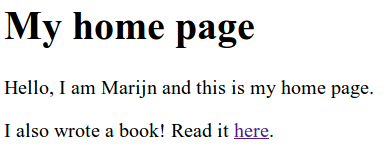
\includegraphics[width=6.3cm]{img/home-page.png}
\vskip 1.5ex\index{HTML!notation}

The tags, wrapped in \index{angle brackets}angle brackets (\lstinline`<` and \lstinline`>`, the symbols for \emph{less than} and \emph{greater than}), provide information about the \index{structure}structure of the document. The other \index{text}text is just plain text.\index{doctype}\index{version}

The document starts with \lstinline`<!doctype html>`, which tells the browser to interpret the page as \emph{modern} HTML, as opposed to various dialects that were in use in the past.\index{head (HTML tag)}\index{body (HTML tag)}\index{title (HTML tag)}\index{h1 (HTML tag)}\index{p (HTML tag)}

HTML documents have a head and a body. The head contains information \emph{about} the document, and the body contains the document itself. In this case, the head declares that the title of this document is ``My home page'' and that it uses the UTF-8 encoding, which is a way to encode Unicode text as binary data. The document's body contains a heading (\lstinline`<h1>`, meaning ``heading 1''—\lstinline`<h2>` to \lstinline`<h6>` produce subheadings) and two \index{paragraph}paragraphs (\lstinline`<p>`).\index{href attribute}\index{a (HTML tag)}

Tags come in several forms. An \index{element}element, such as the body, a paragraph, or a link, is started by an \emph{\index{opening tag}opening tag} like \lstinline`<p>` and ended by a \emph{\index{closing tag}closing tag} like \lstinline`</p>`. Some opening tags, such as the one for the \index{link}link (\lstinline`<a>`), contain extra information in the form of \lstinline`name="value"` pairs. These are called \emph{\index{attribute}attributes}. In this case, the destination of the link is indicated with \lstinline`href="http://eloquentjavascript.net"`, where \lstinline`href` stands for ``hypertext reference''.\index{src attribute}\index{self-closing tag}\index{img (HTML tag)}

Some kinds of \index{tag}tags do not enclose anything and thus do not need to be closed. The metadata tag \lstinline`<meta charset="utf-8">` is an example of this.\index{escaping!in HTML}

To be able to include \index{angle brackets}angle brackets in the text of a document, even though they have a special meaning in HTML, yet another form of special notation has to be introduced. A plain opening angle bracket is written as \lstinline`&lt;` (``less than''), and a closing bracket is written as \lstinline`&gt;` (``greater than''). In HTML, an ampersand (\lstinline`&`) character followed by a name or character code and a semicolon (\lstinline`;`) is called an \emph{\index{entity}entity} and will be replaced by the character it encodes.\index{backslash character!in strings}\index{ampersand character}\index{double-quote character}

This is analogous to the way backslashes are used in JavaScript strings. Since this mechanism gives ampersand characters a special meaning, too, they need to be escaped as \lstinline`&amp;`. Inside attribute values, which are wrapped in double quotes, \lstinline`&quot;` can be used to insert an actual quote character.\index{error tolerance}\index{parsing}

HTML is parsed in a remarkably error-tolerant way. When tags that should be there are missing, the browser reconstructs them. The way in which this is done has been standardized, and you can rely on all modern browsers to do it in the same way.

The following document will be treated just like the one shown previously:

\begin{lstlisting}
<!doctype html>

<meta charset=utf-8>
<title>My home page</title>

<h1>My home page</h1>
<p>Hello, I am Marijn and this is my home page.
<p>I also wrote a book! Read it
  <a href=http://eloquentjavascript.net>here</a>.
\end{lstlisting}
\noindent\index{title (HTML tag)}\index{head (HTML tag)}\index{body (HTML tag)}\index{html (HTML tag)}

The \lstinline`<html>`, \lstinline`<head>`, and \lstinline`<body>` tags are gone completely. The browser knows that \lstinline`<meta>` and \lstinline`<title>` belong in the head and that \lstinline`<h1>` means the body has started. Furthermore, I am no longer explicitly closing the paragraphs since opening a new paragraph or ending the document will close them implicitly. The quotes around the attribute values are also gone.

This book will usually omit the \lstinline`<html>`, \lstinline`<head>`, and \lstinline`<body>` tags from examples to keep them short and free of clutter. But I \emph{will} close tags and include quotes around attributes.\index{browser}

I will also usually omit the \index{doctype}doctype and \lstinline`charset` declaration. This is not to be taken as an encouragement to drop these from HTML documents. Browsers will often do ridiculous things when you forget them. You should consider the doctype and the \lstinline`charset` metadata to be implicitly present in examples, even when they are not actually shown in the text.

\label{browser.script_tag}\section{HTML and JavaScript}\index{JavaScript!in HTML}\index{script (HTML tag)}

In the context of this book, the most important HTML tag is \lstinline`<script>`. This tag allows us to include a piece of JavaScript in a document.

\begin{lstlisting}
<h1>Testing alert</h1>
<script>alert("hello!");</script>
\end{lstlisting}
\noindent\index{alert function}\index{timeline}

Such a script will run as soon as its \lstinline`<script>` tag is encountered while the browser reads the HTML. This page will pop up a dialog when opened—the \lstinline`alert` function resembles \lstinline`prompt`, in that it pops up a little window, but only shows a message without asking for input.\index{src attribute}

Including large programs directly in HTML documents is often impractical. The \lstinline`<script>` tag can be given an \lstinline`src` attribute  to fetch a script file (a text file containing a JavaScript program) from a URL.

\begin{lstlisting}
<h1>Testing alert</h1>
<script src="code/hello.js"></script>
\end{lstlisting}
\noindent

The \emph{code\slash hello.js} file included here contains the same program—\lstinline`alert("hello!")`. When an HTML page references other URLs as part of itself—for example, an image file or a script—web browsers will retrieve them immediately and include them in the page.\index{script (HTML tag)}\index{closing tag}

A script tag must always be closed with \lstinline`</script>`, even if it refers to a script file and doesn't contain any code. If you forget this, the rest of the page will be interpreted as part of the script.\index{relative path}\index{dependency}

You can load \index{ES modules}ES modules (see \hyperref[modules.es]{Chapter 10}) in the browser by giving your script tag a \lstinline`type="module"` attribute. Such modules can depend on other modules by using \index{URL}URLs relative to themselves as module names in \lstinline`import` declarations.\index{button (HTML tag)}\index{onclick attribute}

Some attributes can also contain a JavaScript program. The \lstinline`<button>` tag shown next (which shows up as a button) has an \lstinline`onclick` attribute. The attribute's value will be run whenever the button is clicked.

\begin{lstlisting}
<button onclick="alert('Boom!');">DO NOT PRESS</button>
\end{lstlisting}
\noindent\index{single-quote character}\index{escaping!in HTML}

Note that I had to use single quotes for the string in the \lstinline`onclick` attribute because double quotes are already used to quote the whole attribute. I could also have used \lstinline`&quot;`.

\section{In the sandbox}\index{malicious script}\index{World Wide Web}\index{browser}\index{website}\index{security}

Running programs downloaded from the \index{Internet}Internet is potentially dangerous. You do not know much about the people behind most sites you visit, and they do not necessarily mean well. Running programs by people who do not mean well is how you get your computer infected by \index{virus}viruses, your data stolen, and your accounts hacked.

Yet the attraction of the Web is that you can browse it without necessarily \index{trust}trusting all the pages you visit. This is why browsers severely limit the things a JavaScript program may do: it can't look at the files on your computer or modify anything not related to the web page it was embedded in.\index{isolation}

Isolating a programming environment in this way is called \emph{\index{sandbox}sandboxing}, the idea being that the program is harmlessly playing in a sandbox. But you should imagine this particular kind of sandbox as having a cage of thick steel bars over it so that the programs playing in it can't actually get out.

The hard part of sandboxing is allowing the programs enough room to be useful yet at the same time restricting them from doing anything dangerous. Lots of useful functionality, such as communicating with other servers or reading the content of the copy-paste \index{clipboard}clipboard, can also be used to do problematic, \index{privacy}privacy-invading things.\index{leak}\index{exploit}\index{security}

Every now and then, someone comes up with a new way to circumvent the limitations of a \index{browser}browser and do something harmful, ranging from leaking minor private information to taking over the whole machine that the browser runs on. The browser developers respond by fixing the hole, and all is well again—until the next problem is discovered, and hopefully publicized, rather than secretly exploited by some government agency or \index{mafia}mafia.

\section{Compatibility and the browser wars}\index{Microsoft}\index{World Wide Web}

In the early stages of the Web, a browser called \index{Mosaic}Mosaic dominated the market. After a few years, the balance shifted to \index{Netscape}Netscape, which was then, in turn, largely supplanted by Microsoft's \index{Internet Explorer}Internet Explorer. At any point where a single \index{browser}browser was dominant, that browser's vendor would feel entitled to unilaterally invent new features for the Web. Since most users used the most popular browser, \index{website}websites would simply start using those features—never mind the other browsers.

This was the dark age of \index{compatibility}compatibility, often called the \emph{\index{browser wars}browser wars}. Web developers were left with not one unified Web but two or three incompatible platforms. To make things worse, the browsers in use around 2003 were all full of \index{bug}bugs, and of course the bugs were different for each \index{browser}browser. Life was hard for people writing web pages.\index{Apple}\index{Internet Explorer}\index{Mozilla}

Mozilla \index{Firefox}Firefox, a not-for-profit offshoot of \index{Netscape}Netscape, challenged Internet Explorer's position in the late 2000s. Because \index{Microsoft}Microsoft was not particularly interested in staying competitive at the time, Firefox took a lot of market share away from it. Around the same time, \index{Google}Google introduced its \index{Chrome}Chrome browser, and Apple's \index{Safari}Safari browser gained popularity, leading to a situation where there were four major players, rather than one.\index{compatibility}

The new players had a more serious attitude toward \index{standards}standards and better \index{engineering}engineering practices, giving us less incompatibility and fewer \index{bug}bugs. Microsoft, seeing its market share crumble, came around and adopted these attitudes in its Edge browser, which replaces Internet Explorer. If you are starting to learn web development today, consider yourself lucky. The latest versions of the major browsers behave quite uniformly and have relatively few bugs.
